


Распределения вероятности $P( H0 |D)$, рассчитанные по формуле (3) отдельно для пяти разных моделей, представлены на Рис. \ref{fig:probs}. 

\begin{figure}[H]
\begin{minipage}[h]{0.47\linewidth}
\center{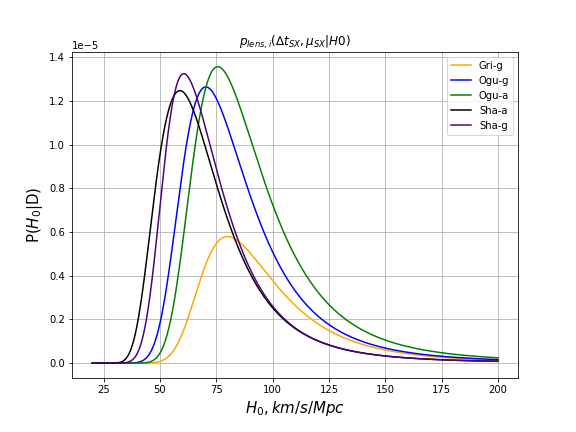
\includegraphics[width=1\linewidth]{hubbleconstant/picsforhubble/SX.png}} a) \\
\end{minipage}
\hfill
\begin{minipage}[h]{0.47\linewidth}
\center{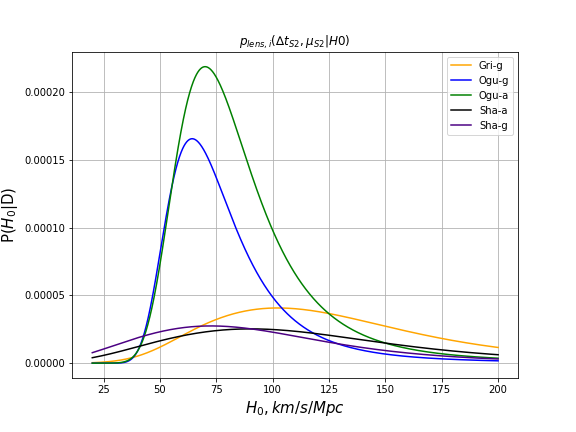
\includegraphics[width=1\linewidth]{hubbleconstant/picsforhubble/S2.png}} \\b)
\end{minipage}
\vfill
\begin{minipage}[h]{0.47\linewidth}
\center{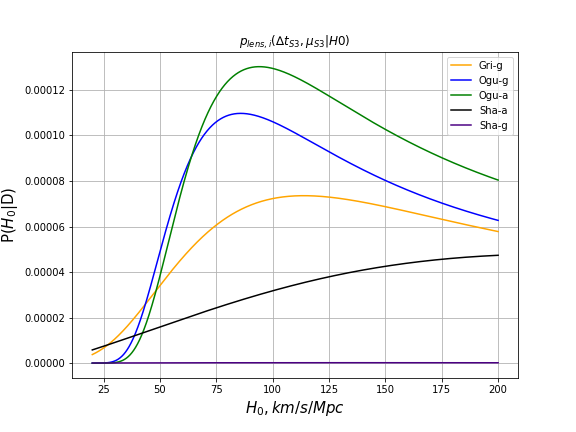
\includegraphics[width=1\linewidth]{hubbleconstant/picsforhubble/S3.png}} c) \\
\end{minipage}
\hfill
\begin{minipage}[h]{0.47\linewidth}
\center{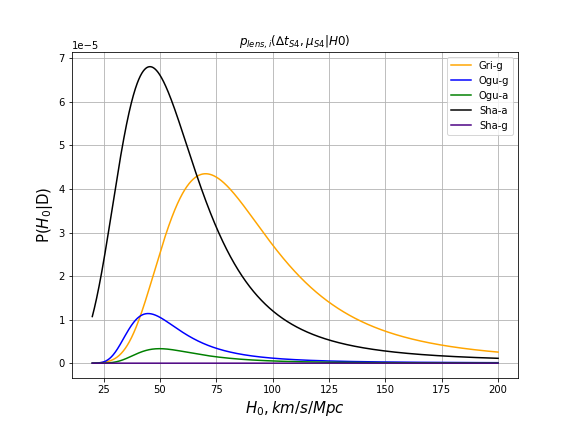
\includegraphics[width=1\linewidth]{hubbleconstant/picsforhubble/S4.png}} d) \\
\end{minipage}
\caption{Вероятность $P( H0 |D)$, вычисленная по формуле (3) для пар изображений SX-S1, S2-S1, S3-S1, S4-S1 (слева направо, сверху вниз). Амплитуда (в относительных единицах) пика указывает на то, насколько хорошо согласуются предсказания усилений, полученных из теоретической модели линзы, с наблюдениями.}
\label{fig:probs}
\end{figure}



Отдельные значения вероятности моделей были сложены с одинаковыми весами. Таким образом были получены распределения $P_+( H0 |D)$ величины постоянной Хаббла, изображенные на Рис. \ref{fig:sumprobs}.

\begin{figure}[H]
\begin{minipage}[h]{0.47\linewidth}
\center{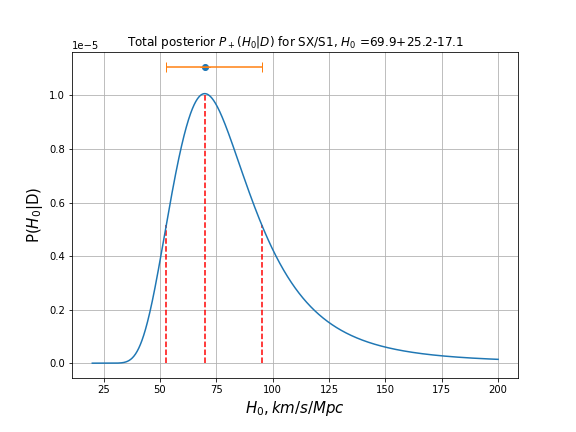
\includegraphics[width=1\linewidth]{hubbleconstant/picsforhubble/H_0 - SX.png}} a) \\
\end{minipage}
\hfill
\begin{minipage}[h]{0.47\linewidth}
\center{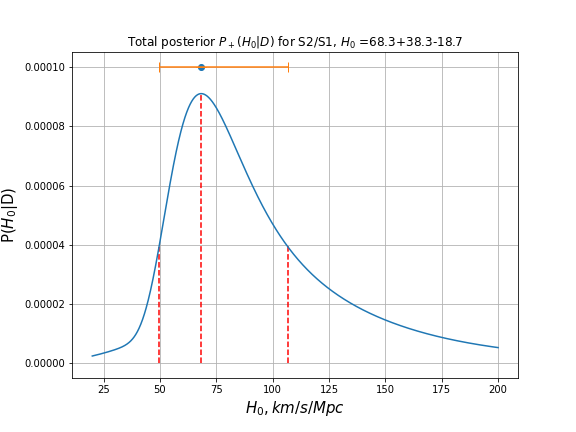
\includegraphics[width=1\linewidth]{hubbleconstant/picsforhubble/H_0 - S2.png}} \\b)
\end{minipage}
\vfill
\begin{minipage}[h]{0.47\linewidth}
\center{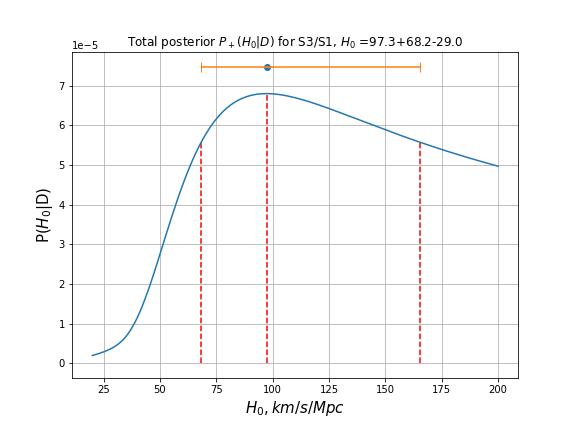
\includegraphics[width=1\linewidth]{hubbleconstant/picsforhubble/H_0 - S3.png}} c) \\
\end{minipage}
\hfill
\begin{minipage}[h]{0.47\linewidth}
\center{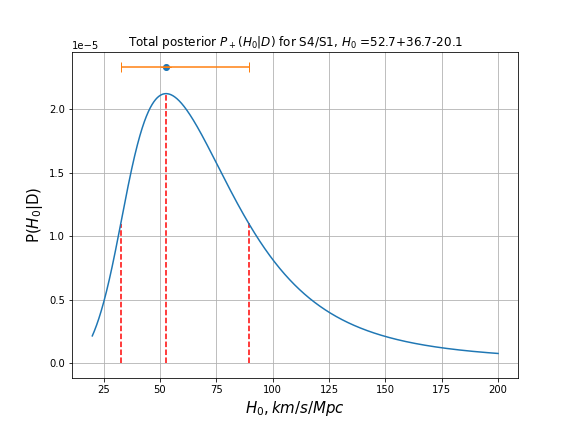
\includegraphics[width=1\linewidth]{hubbleconstant/picsforhubble/H_0 - S4.png}} d) \\
\end{minipage}
\caption{Сумма вероятностей $P_{+}( H_0 |D)$, вычисленных по формуле (3), по всем моделям. В данной работе ошибки рассчитаны относительно пика распределения.}
\label{fig:sumprobs}
\end{figure}




Поскольку область с изображениями S1-S4 находится далеко от области с изображением SX, можно считать, что гравитационные потенциалы в этих областях никак не связаны. Для уменьшения статистических ошибок можно использовать два изображения, которые можно считать нескоррелированными. Поэтому дополнительно значение $H_0$ было рассчитано по комбинации значений, полученных по изображениям S2 и SX. Такой выбор обусловлен тем, что наиболее жёсткие ограничения (то есть самые маленькие ошибки) на временную задержку среди изображений S2, S3, S4 - в изображении S2, как следствие, постоянная Хаббла, вычисленная по ней, будет иметь самые маленькие ошибки. Комбинированная апостериорная вероятность для пары изображений SX-S2 в отдельно взятой модели $i$ вычислялась как

\begin{equation}
p_{lens, i}(\Delta t_{S2},\mu_{S2}|H_0) × p_{lens,i}(\Delta t_{SX}, \mu_{SX}|H_0),
\end{equation}

\noindent после чего полученные значения суммировались с равными для каждой модели весами. Полученные результаты представлены на Рис. \ref{fig:probs2}. Согласно таким оценкам, значение постоянной Хаббла равно $H_0=71.2_ {-11.6}^{+16.4}$. При увеличении числа рассматриваемых гравитационно-линзированных систем можно существенно улучшить ошибки величины $H_0$.

\begin{figure}[h]
\begin{minipage}[h]{0.49\linewidth}
\center{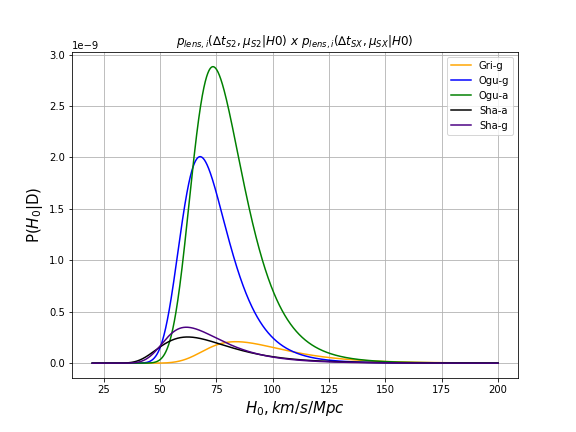
\includegraphics[width=0.99\linewidth]{hubbleconstant/picsforhubble/SX+S2.png}}
\end{minipage}
\hfill
\begin{minipage}[h]{0.49\linewidth}
\center{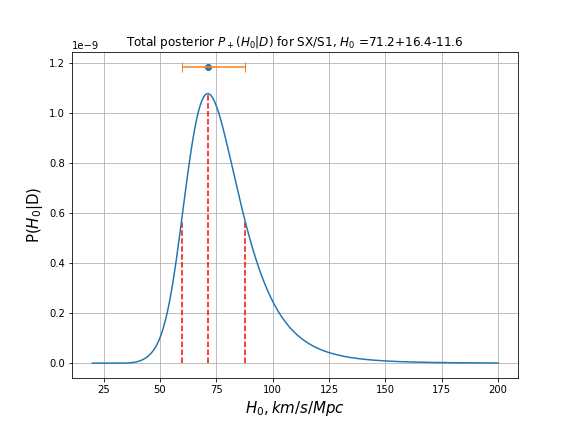
\includegraphics[width=0.99\linewidth]{hubbleconstant/picsforhubble/H_0 - SX+S2.png}}
\end{minipage}
\caption{Слева: $P( H0 |D)$ для изображений SX и S2 для отдельно взятых моделей, рассчитанная по формуле (4). Справа: сумма вероятностей $P_{+}( H0 |D)$ по всем моделям.}
\label{fig:probs2}
\end{figure}



\section{Обсуждение}

На основе сравнения прогнозов временных задержек и коэффициентов усиления, рассчитанных в различных моделях гравитационного потенциала линзы-галактики и масштабированных таким образом, чтобы они совпадали с наблюдаемыми величинами, вычислено значение постоянной Хаббла, наиболее точно удовлетворяющее и модельным, и наблюдательным данным: $H_0=71.2_ {-11.6}^{+16.4}$ . Для уменьшения статистических ошибок это значение было рассчитано по нескольким изображениям сверхновой SN Refsdal. Существенно улучшить оценку $H_0$ поможет увеличение числа рассматриваемых систем. Полученные результаты также могут послужить независимым тестом различных  моделей распределения масс в линзе-галактике. Также следует отметить, что при вычислениях не учитывалось влияние микролинзирования. Этот эффект рассмотрен в следующем разделе.
